\documentclass{article}
\usepackage[margin=.2in]{geometry}
\usepackage[sfdefault]{roboto}
\usepackage[T1]{fontenc}
\usepackage{graphicx}

\begin{document}
\pagenumbering{gobble}

\noindent \textbf{Supplemental Figure S3.}
Densities of top four enriched motifs at ends of chromosomal \textbf{(A)} \textit{p} arms and \textbf{(B)} \textit{q} arms of the HG004 dataset (Ashkenazim trio, mother).
Only the arms covered by at least 25 reads are displayed.
Genomic coordinates are given in Kbp.
Vertical red dashed lines denote the position of the boundary of the annotated telomeric tract.

\begin{figure}[h] \centering
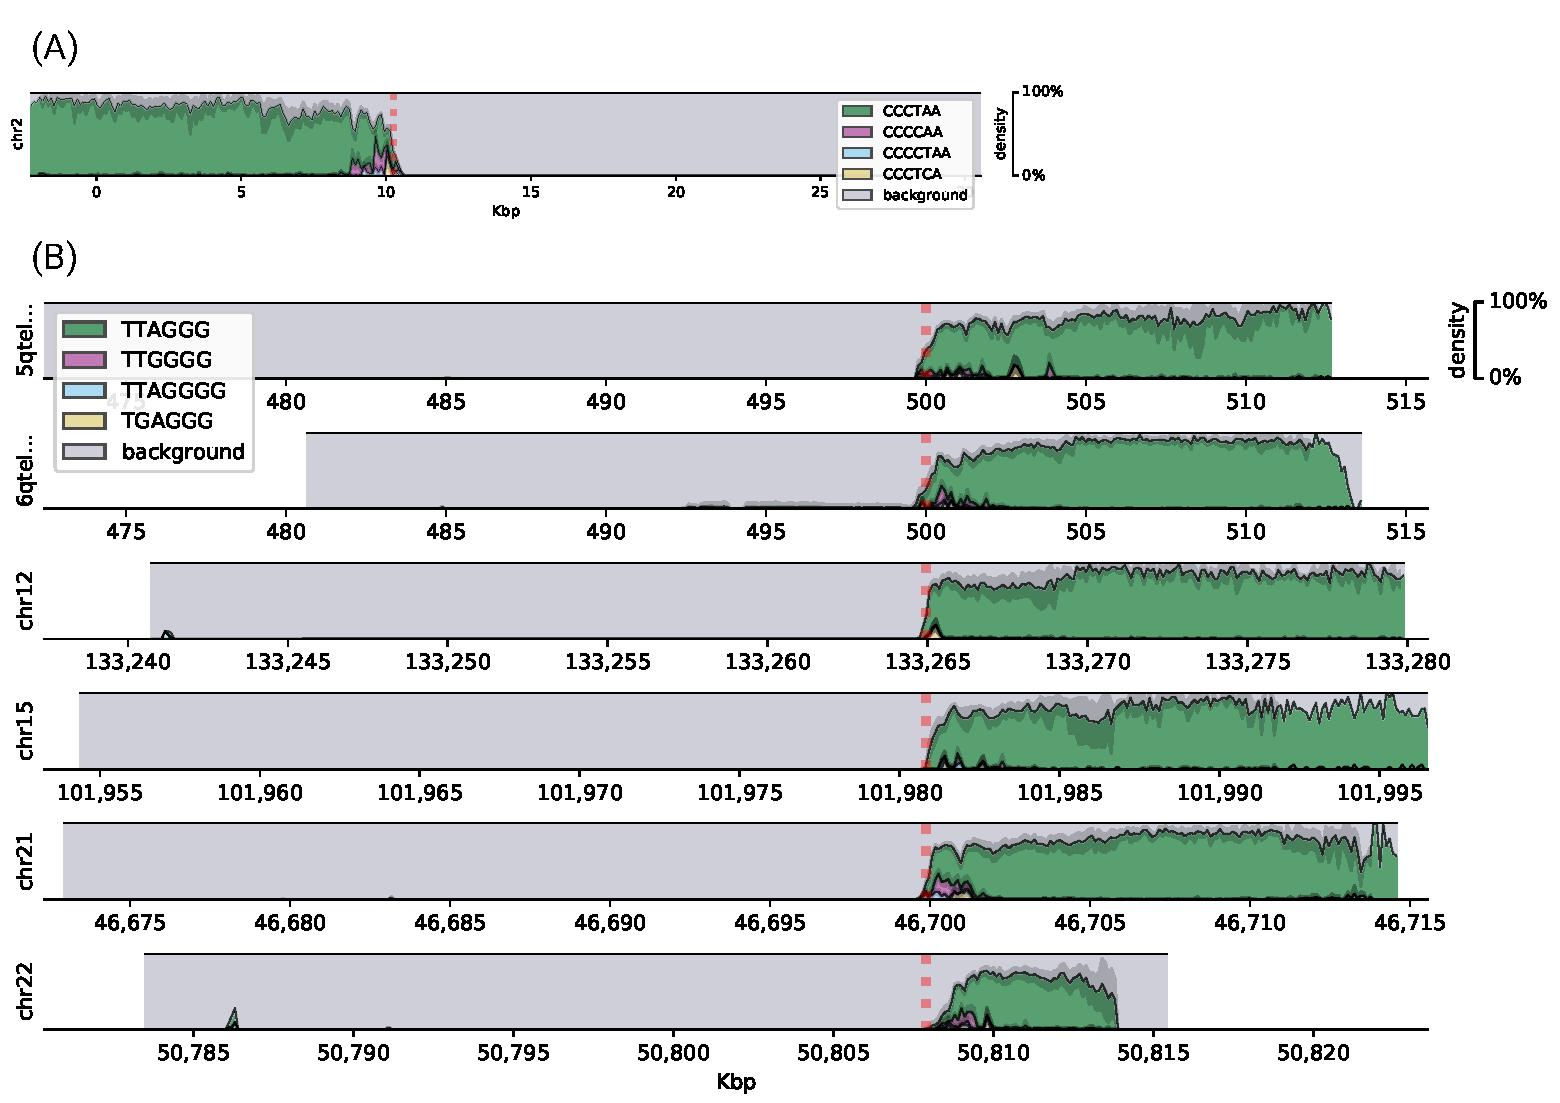
\includegraphics[width=\textwidth,keepaspectratio]{renders/figures/Figure-S3.pdf}
\end{figure}

\end{document}
